\documentclass[11pt]{article}
\usepackage[T1]{fontenc}
\usepackage[a4paper,margin=2.5cm]{geometry}
\usepackage{graphicx}
\usepackage{amsmath}
\usepackage[backend=biber,style=authoryear]{biblatex}
\usepackage{hyperref}
\graphicspath{{img/}}
\addbibresource{references.bib}

\title{Gradient Descent on Noisy Objectives:\\ A Short Empirical Note}
\author{B. Researcher}
\date{}

\begin{document}
\maketitle

\begin{abstract}
We compare plain gradient descent with two variants on objectives whose
gradients carry random noise. Momentum helps when the noise is small and
hurts when it dominates; averaging the iterates helps in both cases.
\end{abstract}

\section{Introduction}
Stochastic optimisation goes back to \textcite{robbins51}. Modern training
methods add momentum \parencite{polyak64} or adaptive step sizes
\parencite{kingma15}. This note asks a narrow question: on a simple quadratic
with noisy gradients, which variant reaches a small error first?

\section{Method}
We minimise $f(x) = \tfrac12 \lVert A x - b \rVert^2$ with gradient estimates
\begin{equation}
  g_t = A^\top (A x_t - b) + \sigma \varepsilon_t,
  \qquad \varepsilon_t \sim \mathcal{N}(0, I).
\end{equation}
Figure~\ref{fig:overview} sketches the experiment grid: three noise levels
times three methods, ten seeds each.

\begin{figure}[ht]
  \centering
  
\includegraphics[width=0.45\textwidth]{overview}
  \caption{The experiment grid.}
  \label{fig:overview}
\end{figure}

\section{Results}
Figure~\ref{fig:convergence} shows the error over the first two hundred
steps for the middle noise level. Iterate averaging reaches the target error
in about half the steps of plain descent, as the theory of
\textcite{polyak92} predicts.

\begin{figure}[ht]
  \centering
  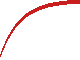
\includegraphics[width=0.45\textwidth]{plots/convergence}
  \caption{Error against step count, $\sigma = 0.1$.}
  \label{fig:convergence}
\end{figure}

\section{Discussion}
The setting is small on purpose. The ranking may change on non-convex
objectives, and we make no claim about them.

\printbibliography

\end{document}
